Writing programs that control lights and motors is fun, but to build really interesting creations we need to be able to respond to events in the world. In the next few chapters, we'll learn how to respond to events that take place in the world around us.

\GOALS
Connect a button to the Arduino and use it to turn an LED on and off.

\section{The Circuit}
For this circuit, we'll add a button to the Arduino that lets us turn an LED on and off. To do this, we'll need to see how to attach a button to the Arduino.

You will need:
\begin{enumerate}
	\item Your Arduino
	\item A button
	\item A 10k\ohm resistor
	\item Some jumper wire
	\item An LED and a 470\ohm resistor
\end{enumerate}

A picture of what you're going to build (and the circuit diagram) can be found in Figure~\vref{diagram:ch4-button-circuit}.

\begin{figure}[ht]
  \begin{center}
    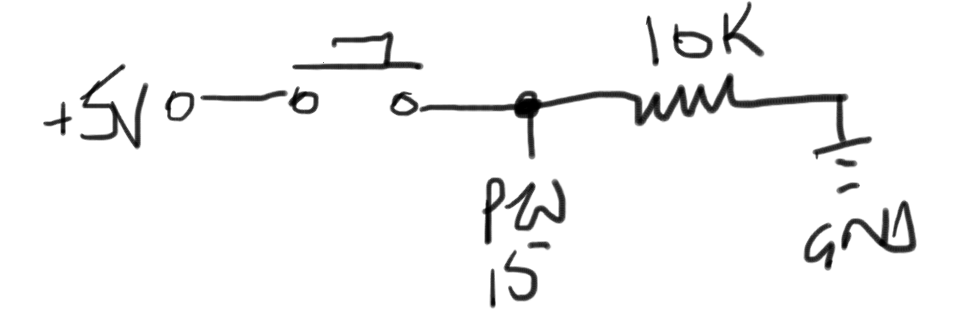
\includegraphics[width=0.8\linewidth]{images/ch4-button-circuit}
    \caption{Connecting a button to the Arduino.}
    \label{diagram:ch4-button-circuit}
  \end{center}
\end{figure}

The newest and most interesting part of this circuit is the addition of the button. One leg of the button will be connected to the {\code +5V} pin on the Arduino. The opposite leg will be connected to ground through a 10k\ohm resistor (\resistor{Brown}{Black}{Orange}, Brown Black Orange Gold). From the same column as the resistor we will connect a wire to pin \pintwo on the Arduino; we will use pin \pintwo to detect whether the button has been pressed. 

Getting this circuit wrong could have some unpleasant consequences for your Arduino. Remember, there are plenty of texts that will teach you more about electronics than this one. That said, you should know why that 10k\ohm resistor is so important. If you left it out, pushing the button would be equivalent to connecting {\code +5V} directly to pin \pintwo. Why is this bad? The only resistance between the voltage source and pin \pintwo would be the resistance of the wire; it turns out that this is a very small number. If we look at Ohm's Law\footnote{XXX Wikipedia link}, we see why this is bad.

%\begin{equation}
%	V = IR
%\end{equation}

\begin{figure}[ht]
  \begin{center}
    
\includegraphics[width=0.8\linewidth]{images/ch4-ohms-law}
    %\caption{Connecting a button to the Arduino.}
    \label{image:ohms-law}
  \end{center}
\end{figure}

If the resistance is very small, and the voltage is constant ({\code +5V}), then the current must be big. Resistors limit the current flow in a circuit; without it, we would sink more current into pin \pintwo than the Arduino can handle, frying our processor. By including the resistor---specifically, a pretty big one---the current drops a great deal, and pressing the button does not mean death for pin \pintwo.

\newpage

\section{Pictures and Code}

Programming is an incredibly visual activity. If you observe two experienced programmers discussing a programming problem, you'll discover that they make heavy use of diagrams in their conversation. When we're working with \occam, we also make heavy use of diagrams. This is especially nice because we can translate those diagrams directly into code.


\begin{figure}[ht]
  \begin{center}
    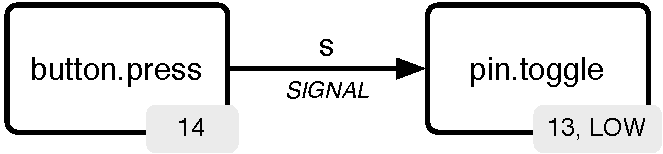
\includegraphics[width=0.8\linewidth]{images/ch4-button-toggle-led}
    \caption{A communicating two-process network.}
    \label{diagram:ch4-button-toggle-led}
  \end{center}
\end{figure}

We call this a {\strong process network}. Each large box represents a {\strong process}, which is a piece of code that is churns away independently of every other process. We use small, gray boxes to indicate {\strong parameters} that adjust the alter the behavior of the process they are attached to. So, in Figure~\vref{diagram:ch4-button-toggle-led}, we would say that {\code button.press} has one parameter, which is {\constant 14}. 

The arrow between the two processes is a \CHANnel. Specifically, it is a communications channel---a wire---that connects one process to another. When we look at Figure~\vref{diagram:ch4-button-toggle-led}, we can tell that the process {\code button.press} communicates over a channel called {\code s} with a process called {\code pin.toggle}. We know that {\code pin.toggle} does {\em not} talk with {\code button.press}, simply because the arrow tells us which way the communications take place.


\subsection{From pictures to code}
We can, by following a few simple rules, convert the diagram on page ~\pageref{diagram:ch4-button-toggle-led}\xspace into code. {\strong All the information we need to write a valid \occam program is contained in the process network diagram.} It is a lot more fun to design programs  when you can do it visually in a sketchbook as opposed to in front of a screen.

First, we see there are two {\strong processes}. We can write down their names.

\vspace{3mm}
\begin{lstlisting}
button.press()
pin.toggle()
\end{lstlisting}

Next, we know that both processes have {\strong parameters} associated with them (the gray boxes). We're going to need to include those parameters in our code%\footnote{Because these processes are part of the \plumbing library, we do have to make sure the parameters go in the right place... if you juggle them around randomly, you will get an error}
.

\vspace{3mm}
\begin{lstlisting}
button.press(14)
pin.toggle(13, LOW)
\end{lstlisting}

Because there is an arrow connecting these two processes, we're going to need a \CHANnel to communicate over. But here's the trick: {\strong all communications must happen in \PARallel}. Why? Can you have a phone conversation with someone where you speak and {\em then} they listen? Or, do they have to be listening {\em at the same time} as you are speaking? See. 

{\strong Communications must happen in \PARallel.}

\newpage

To run our two processes in parallel, we put them under a \PAR. Remember that everything underneath a \PAR gets indented by two spaces!

\vspace{3mm}
\begin{lstlisting}
PAR
  button.press(14)
  pin.toggle(13, LOW)
\end{lstlisting}

We're only missing one thing at this point: the \CHANnel. We have to {\strong declare} the channel outside the \PAR. What this means is that we have to tell \occam that we want a communications channel (we'll call it {\code s}). Further, we have to tell \occam what {\em kind} of information it will carry. In this case, we want it to carry information of type \SIGNALT. 

The declaration looks like this:

\vspace{3mm}
\begin{lstlisting}
CHAN SIGNAL s:
PAR
  button.press(14)
  pin.toggle(13, LOW)
\end{lstlisting}

By placing the declaration before the \PAR, it indicates that the processes that are running in parallel may, if they wish, use the channel {\code s} to send a \SIGNALV. Now we have just one step left: we have to give one end of the channel to each of the two processes in the \PAR.

\newpage

A channel is a lot like soup cans on string: one person talks, and the other listens. Unlike soup cans on string, you can't take turns talking and listening at both ends: there's just one talking end, and just one listening end, and that's it.

\begin{wrapfigure}{r}{0.5\linewidth}
	  \begin{center}
    	
\includegraphics[width=0.8\linewidth]{images/ch4-sending-receiving}
			%\captionsetup{labelformat=empty,justification=centering,font=footnotesize}
%\caption{A good resource.}
    	%\label{screenshot:compile-successful}
  \end{center}
\end{wrapfigure}

\ \\

\vspace{3mm}
The talking (or {\strong sending}) end of a channel is marked with a {\code !}. The exclamation point (or {\em bang}, from British English) tells \occam which end of the channel is sending information. It's as if that end of the channel is shouting: ``Hey! Hey you! I've got a \SIGNALV for you!''

\vspace{3mm}
The listening (or {\strong receiving}) end of a channel is marked with a {\code ?}. The question mark (or {\em eh?}, from Canadian English) tells \occam which end of the channel is receiving information. It's as if that end of the of the channel is waiting for instructions: ``Eh? Come again? What did you say?''

\clearpage
\newpage

Lastly, wrap your code in a \PROCedure called {\code main}, and indent everything another two spaces. (We don't get that step from the diagram.) When you're done, your program should look like this:

\vspace{3mm}
\lstinputlisting[caption=Using a button to toggle an LED on and off.,label=code:button-toggle-led]{code/button-toggle-led.occ}

\subsection{In summary}
%There is a great deal more we could say about processes, channels, and how they communicate data between them. However, we won't say it right now. Instead, we want you to explore this code a bit, see how you can break it, and then keep moving forward. We'll continue to explain how and why \plumbing works the way it does in future chapters.

To summarize what we learned in this chapter:


\begin{itemize}
	\item Each box in the diagram represents a \PROCedure. Because there are two boxes in the diagram, we can expect to find a \PAR in our code with two processes indented underneath it. 
	\item The two processes are connected by a single \CHANnel. A channel carries information in one direction only, from one process to another. In this chapter, the channel's name was {\code s}.
	\item Each process may take some parameters; in this chapter, the process called \bp takes a pin number; the process \tp takes both a pin number as well as whether it should start out \LOW or \HIGH.
\end{itemize}


\BREAKAGE
There are lots of ways to break the code in this chapter, as usual.

\begin{description}		
	\item[Forget the colon]\ \\
	At the end of the \CHANnel declaration, remove the colon. What happens? This is a common error made by many.
	\item[Indent the PAR]\ \\
	What happens if you indent the \PAR two spaces under the \CHAN? We suspect this makes \plumbing unhappy. This is rather common as errors go as well.

	\item[Swap {\code !} and {\code ?}]\ \\
	Try switching the location of the {\code !} and {\code ?}. 
	
	\item[Leave out the {\code !} and {\code ?}]\ \\
	Try it. As it happens, this isn't an error. Perhaps it should be?
	
	\item[Forget the \SIGNALT]\ \\
	When we write \CHAN \ \SIGNALT \ {\code s}, we are telling \plumbing that the channel carries information of the type \SIGNALT over the channel {\code s} and nothing else. What happens if you delete the word \SIGNALT?
	
	\item[Forget the {\code s}]\ \\
	When we write \CHAN \ \SIGNALT \ {\code s}, we are telling \plumbing that the channel is named {\code s}. What happens if you remove the letter {\code s}?
		
\end{description}




%%%%%%%%%%%%%%%%%%%%%%%%%%%%%%%%%%%%%%%%%%%%%%%%%%%%%%%
% MATERIAL PULLED... NOT BAD, JUST NOT USED HERE.
%%%%%%%%%%%%%%%%%%%%%%%%%%%%%%%%%%%%%%%%%%%%%%%%%%%%%%%


\begin{comment}


\subsection{Test it!}
If you've assembled your circuit correctly, you should be able to run the program from this chapter and use the button to turn the built-in LED on and off!

\PATTERNS
% We? You? Need to get this straight throughout the text. Make a decision. Are we talking with them, or two them, or do we avoid this kind of language all together?
In the previous chapter, we saw how to run two processes in \PARallel. Specifically, we were able to blink two LEDs at the same time, and (if we wanted), both could blink at different rates. However, the rate of one LED did not, in any way, affect the blink rate of the other LED.

In this program, the button is clearly turning the LED on and off. To do this, we've built our first {\em process network}. That is, we have more than one process that is executing in parallel, and one is communicating information to the other.

%Perhaps intro some diagrams in chapter 3, since it is so light-weight at the moment?
\subsection{A two-process network}
\plumbing is all about connecting one parallel process up to another and communicating information between those processes. This turns out to be a highly visual notion, so we like to draw pictures of our process networks whenever possible.
 
\begin{figure}[ht]
  \begin{center}
    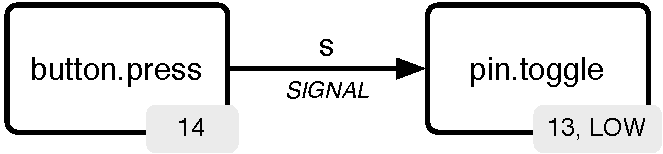
\includegraphics[width=0.8\linewidth]{images/ch4-button-toggle-led}
    \caption{A communicating two-process network.}
    \label{diagram:ch4-button-toggle-led-also}
  \end{center}
\end{figure}

This diagram tells us a great deal about the \plumbing program that we're writing. We'll repeat that here, so you don't have to flip pages:

\lstinputlisting[caption=The code and diagram are related.]{code/button-toggle-led.occ}

\begin{itemize}
	\item Each box in the diagram represents a process. Because there are two boxes in the diagram, we can expect to find a \PAR in our code with two processes indented underneath it. 
	\item The two processes are connected by a single \CHANnel. A channel carries information in one direction only, from one process to another. In this diagram, the channel's name is {\code s}.
	\item Each process takes some other parameters; in this case, the process called \bp takes a pin number; the process \tp takes both a pin number as well as whether it should start out \LOW or \HIGH.
\end{itemize}

Process network diagrams are a good way to think about \plumbing programs. We will see many more pictures of process networks, and will see how they are converted into code time and again. This is your first introduction, and we'll spiral deeper into these ideas in the coming chapters.

\subsection{The channel}
We need a \CHANnel to share information from one process to another in a \plumbing program. Actually, it is the {\em only} way to get information from one process to another. When you want to use a channel, you first have to {\strong declare} that channel in your code. The pattern for declaring a channel can be found in Figure~\vref{diagram:pattern-channel-decl}.

\begin{figure}[ht]
  \begin{center}
    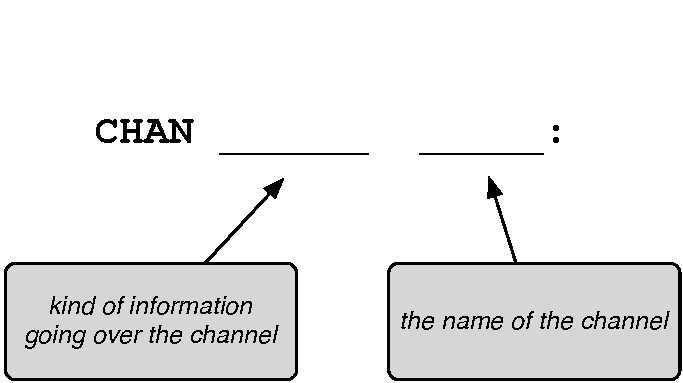
\includegraphics[width=0.6\linewidth]{images/ch4-pattern-channel-decl}
    \caption{How to declare a channel.}
    \label{diagram:ch4-pattern-channel-decl}
  \end{center}
\end{figure}

The first blank contains the {\em kind} of information that is going over the channel. If you prefer, you can think of each channel as having a particular shape, and only information that matches that shape can travel through the channel. In this chapter's code, we are sending a \SIGNALV over the channel---think of it as a sonar ping that a submarine might emit.

The second blank is the {\em name} of the channel. As the programmer, you get to choose the channel name. When we are naming channels within a \PROC, we will typically give them single-letter names. So, this channel is named {\code s}. 

The last thing to note about declaring a channel is that it typically comes before a \PAR. When we do this, every process indented under the \PARallel block then has access to the channel. This does not mean that every process in the block may {\em use} the channel. This is because every channel has two ends: a sending end, and a receiving end.

\subsubsection{How communication works}

\begin{figure}[ht]
  \begin{center}
    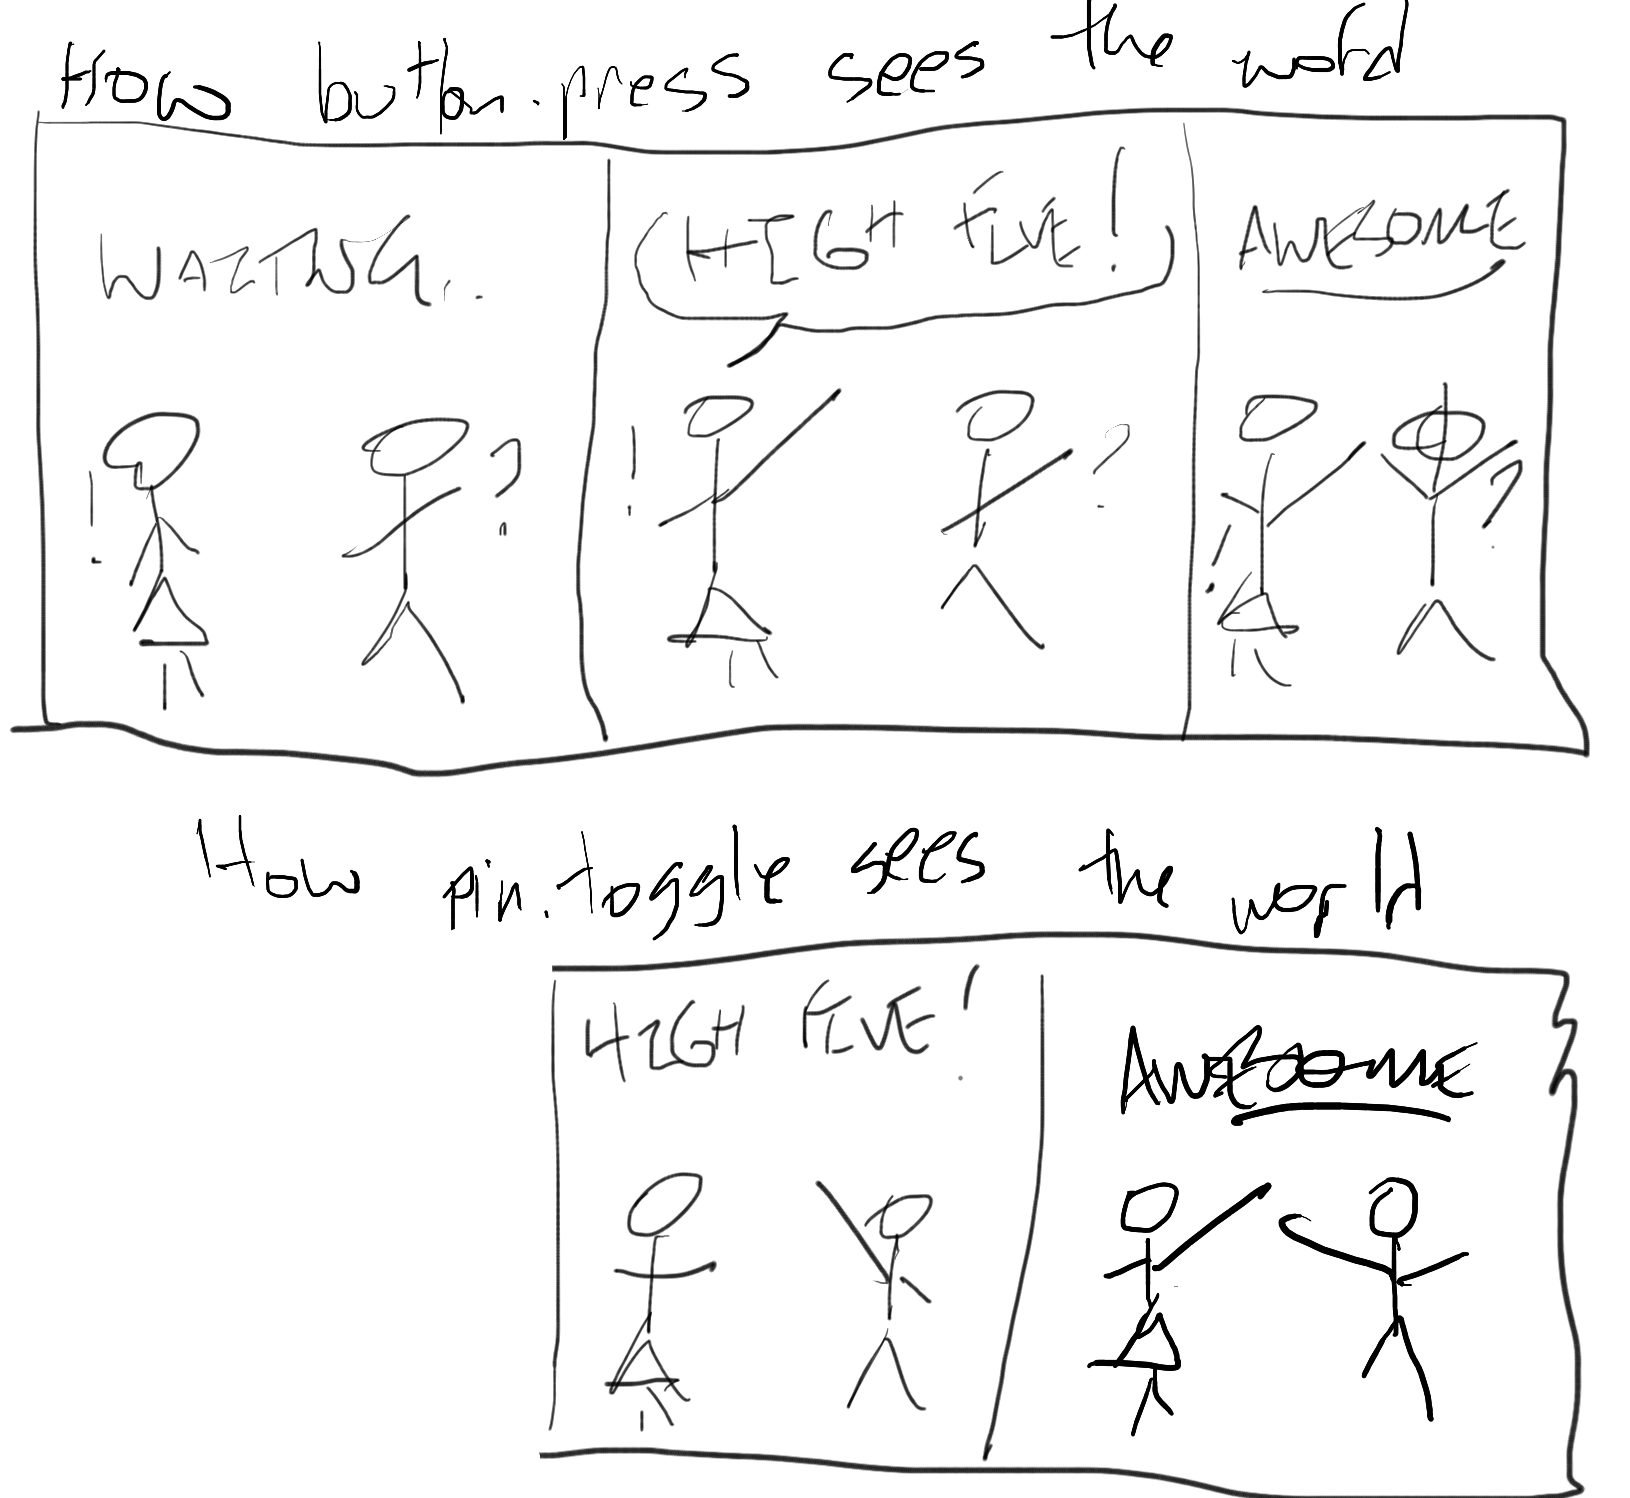
\includegraphics[width=0.8\linewidth]{images/ch4-high-five-channel-comms}
    \caption{Channel communication is like a high-five.}
    \label{diagram:ch4-high-five-channel-comms}
  \end{center}
\end{figure}

Channel communication is like giving your friend a high-five (Figure~\vref{diagram:high-five-channel-comms}).


The process \bp sits around waiting for you to press the button. When you do, it says ``high five!'' over the channel {\code s}. It then waits until \tp gets around to completing the high five, at which point the \SIGNALV has been passed from one process to another. (This, of course, is awesome.)

From the point of view of the \tp process, it says ``high five?,'' and hopes that \bp won't leave it hanging. However, \tp will wait forever, if necessary, for a \SIGNALV from \bp. When you get around to pushing the button on the Arduino, \bp completes the high five with \tp, and your LED turns on or off.


\subsubsection{The sending end of a channel}
The \bp process holds the sending end of the channel. That is because we want a \SIGNALV sent to the \tp process whenever the button is pressed. To make it clear that \bp holds the sending end of the channel, we provide the channel as a parameter to the process, but put an exclamation point after the channel name. Think of it as shouting: the \bp process will be shouting! some information to the process at the other end of the channel.

\subsubsection{The receiving end of a channel}
The \tp process is listening for a signal. It will wait all day if necessary, and until it hears a message on the channel, it won't do anything. That is why the parameter {\code s?} has a question mark: it means that \tp is saying ``what? huh?,''waiting for \bp to send it a message.

\subsection{A few quick words}
Just a few quick words about the other new things in this chapter's code.

\subsubsection{A quick word about \LOW and \HIGH}
We thought we should mention this briefly: there is a reason we do not say {\code ON} and {\code OFF} in our code. You see, LEDs turn on at a specific voltage, but it isn't 5V. It is actually somewhere inbetween 0V and 5V, and it is a little different for every LED. For that reason, we say that we drive a pin \LOW when we take it down near 0V, and we drive a pin \HIGH when we take it up near 5V. So, to turn an LED on, we drive its pin \HIGH; to turn it off, we drive that pin \LOW. Why people call it ``driving a pin'' is another thing entirely.

\subsubsection{A quick word about the dot in \bp}
The {\code .} in \bp doesn't mean anything. It is how, in \plumbing programs, we insert a space into the name of a process. You see, you can't use spaces, so we use a dot. (If you're familiar with Java, please forget everything you have ever learned about the dot. It doesn't apply here.)

\subsubsection{Channel ends as parameters}
Up until now, you have only seen numbers as parameters. Channel ends can be parameters, too. Otherwise, how would one process talk to another?

\subsubsection{\LOW and \HIGH as parameters}
\LOW and \HIGH are what we call {\em constants}. They get converted into numbers when you send your program to the Arduino. So, instead of putting ``magic numbers'' in your code (which you might forget the meaning of), you can use \LOW and \HIGH anywhere that we might talk about whether we should drive a pin to full voltage or zero voltage.

\end{comment}


	
	
